%%%%%%%%%%%%%%%%%%%%%%%%%%%%%%%%%%%%%%%%%
% University Assignment Title Page 
% LaTeX Template
% Version 1.0 (27/12/12)
%
% This template has been downloaded from:
% http://www.LaTeXTemplates.com
%
% Original author:
% WikiBooks (http://en.wikibooks.org/wiki/LaTeX/Title_Creation)
%
% License:
% CC BY-NC-SA 3.0 (http://creativecommons.org/licenses/by-nc-sa/3.0/)
% 
% Instructions for using this template:
% This title page is capable of being compiled as is. This is not useful for 
% including it in another document. To do this, you have two options: 
%
% 1) Copy/paste everything between \begin{document} and \end{document} 
% starting at \begin{titlepage} and paste this into another LaTeX file where you 
% want your title page.
% OR
% 2) Remove everything outside the \begin{titlepage} and \end{titlepage} and 
% move this file to the same directory as the LaTeX file you wish to add it to. 
% Then add \input{./title_page_1.tex} to your LaTeX file where you want your
% title page.
%
%%%%%%%%%%%%%%%%%%%%%%%%%%%%%%%%%%%%%%%%%
%\title{teoriadeinformacao}
%----------------------------------------------------------------------------------------
%	PACKAGES AND OTHER DOCUMENT CONFIGURATIONS
%----------------------------------------------------------------------------------------

\documentclass[12pt]{article}
\usepackage[english]{babel}
\usepackage[utf8x]{inputenc}
\usepackage{amsmath}
\usepackage{graphicx}
\usepackage[colorinlistoftodos]{todonotes}
\usepackage{placeins}
\usepackage{makeidx}

\makeindex


\begin{document}

\begin{titlepage}

\newcommand{\HRule}{\rule{\linewidth}{0.5mm}} % Defines a new command for the horizontal lines, change thickness here

\center % Center everything on the page
 
%----------------------------------------------------------------------------------------
%	HEADING SECTIONS
%----------------------------------------------------------------------------------------

\textsc{\LARGE Universidade de Évora}\\[1.5cm] % Name of your university/college
\textsc{\Large Disciplina de Teoria de Informação}\\[0.5cm] % Major heading such as course name
%\textsc{\large Minor Heading}\\[0.5cm] % Minor heading such as course title

%----------------------------------------------------------------------------------------
%	TITLE SECTION
%----------------------------------------------------------------------------------------

\HRule \\[0.4cm]
{ \huge \bfseries Compressão, Descompressão e Capacidade de canais discretos sem memória}\\[0.4cm] % Title of your document
\HRule \\[1.5cm]
 
%----------------------------------------------------------------------------------------
%	AUTHOR SECTION
%----------------------------------------------------------------------------------------

\begin{minipage}{0.4\textwidth}
\begin{flushleft} \large
\emph{Autor:}\\
Marcus \textsc{Santos}, 29764\\
Ricardo \textsc{Fusco}, 29263
\end{flushleft}
\end{minipage}
~
\begin{minipage}{0.4\textwidth}
\begin{flushright} \large
\emph{Professor:} \\
Miguel \textsc{Barão}
\end{flushright}
\end{minipage}\\[2cm]

% If you don't want a supervisor, uncomment the two lines below and remove the section above
%\Large \emph{Author:}\\
%John \textsc{Smith}\\[3cm] % Your name

%----------------------------------------------------------------------------------------
%	DATE SECTION
%----------------------------------------------------------------------------------------

{\large \today}\\[2cm] % Date, change the \today to a set date if you want to be precise

%----------------------------------------------------------------------------------------
%	LOGO SECTION
%----------------------------------------------------------------------------------------


\includegraphics[scale=0.5]{uevora.png}\\[1cm] % Include a department/university logo - this will require the graphicx package
 
%----------------------------------------------------------------------------------------

\vfill % Fill the rest of the page with whitespace

\end{titlepage}

\newpage
\thispagestyle{empty}
\renewcommand\contentsname{Índice}
\tableofcontents
\newpage
\renewcommand\listfigurename{Lista de Figuras}
\listoffigures
\newpage
\index{Introdução}

\printindex
\section{Introdução}

No contexto da disciplina de Teoria de Informação pretende-se, através de um dos algoritmos de compressão abordados ao longo da disciplina, comprimir e descomprimir uma imagem no formato PBM (Portable Bitmap Image). Para tal é necessário efectuar uma análise de dados acerca do ficheiro a comprimir para conseguir uma melhor compressão. Para além das funções necessárias para a compressão/descompressão, como o cálculo das frequências de cada simbolo de acordo com o tamanho do grupo utilizado, a construção da árvore e dos códigos para cada símbolo, é também necessário o calculo das diferentes entropias, informação mútua, distribuição estacionária, taxas de compressão, etc, com o intuito de estabelecer relações e retirar conclusões relativamente aos dados observados. O algoritmo de compressão de dados sem perdas seleccionado para este trabalho é o algoritmo de Huffman. Escolhemos este algoritmo pois, de acordo com a nossa opinião, é o que se adequa melhor para a compressão deste tipo de dados visto sabermos já à priori as probabilidades p(x) e tendo em conta que o código de Huffman é o melhor código instantâneo que poderia ser construido para um determinado alfabeto. \\
\\A segunda parte do trabalho consistirá em criar um programa que, através do algoritmo de Blahut, calcule a capacidade do canal aproximada para canais discretos sem memória. A linguagem de programação que iremos utilizar ao longo do trabalho será Python. \\

\newpage

\section{Compressão}
 Tal como referenciado anteriormente o algoritmo de compressão escolhido na implementação do trabalho foi o algoritmo de Huffman. Este tira partido da probabilidade de ocorrer um símbolo no ficheiro para assim construir códigos de tamanho variável onde os simbolos com menor probabilidade irão ser agrupados e reordenados segundo as suas frequências, ou seja, os simbolos com maior probabilidade irão ter um codigo com menor tamanho, conseguindo assim uma taxa de compressão próxima da entropia, ou seja, perto do limite máximo de compressão de dados sem perda de informação.\\
 \\
 O ficheiro comprimido contém duas partes distintas onde uma delas possui a informação para descomprimir o ficheiro através da reconstrução da árvore de Huffman e a segunda parte são os dados comprimidos. A primeira parte, designada header, é composta pelo grupo(sequência de bits que irá ser agrupada), pelo número zeros adicionados no fim do ficheiro(para o caso de o resto da divisão do tamanho do ficheiro pelo tamanho do grupo seja diferente de zero) e o percurso em pós-ordem na árvore de Huffman. A segunda parte contém os dados comprimidos através dos códigos gerados pela da árvore de Huffman.\\
\subsection{Estrutura do ficheiro comprimido}
O  ficheiro comprimido é composto por duas partes onde a primeira contém todos os dados necessário para descodificar a imagem pbm, nomeadamente o tamanho do grupo utilizado, o número de zeros acrescentados no fim do ficheiro e o percurso pós-ordem da árvore de Huffman\\
\newpage



\subsection{Árvore de Huffman}
A codificação de Huffman utiliza uma árvore binária e as frequências dos símbolos ocorridos no ficheiro para construir os códigos que serão utilizado para comprimir a imagem em formato pbm. Mas antes de começar a verificar a ocorrência dos símbolos no ficheiro é necessário escolher o tamanho do grupo que irá formar um símbolo. Ao determinar o tamanho desse grupo, ou seja, a sequência de bits que irá perfazer um símbolo, sabe-se também quantos símbolo existem. A seguir procede-se à análise das frequência dos símbolos no ficheiro. Todos os simbolos são folhas de uma árvore de Huffman\\
\\
Com as frequências calculadas já é possível construir então a árvore de Huffman e criar os códigos a partir da mesma.\\
\\
A imagem seguinte representa gráficamente um exemplo de uma árvore de Huffman onde as folhas dessa árvore são as ocorrências de um caracter numa determinada sequência de caracteres\\

\begin{figure}[h]
  \caption{Representação da árvore de Huffman}
  \centering
    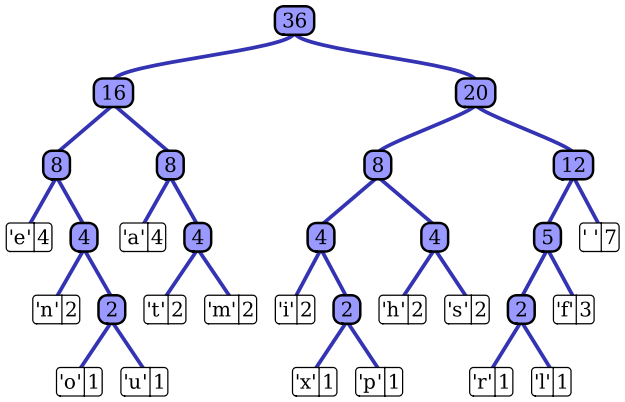
\includegraphics[width=0.7\textwidth]{huffman.png}
\end{figure}


\subsubsection{Estrutura de dados utilizada para representar a árvore de huffman}

Ao longo do desenvolvimento do trabalho foram utilizadas duas estruras para representar a árvore. Uma delas é uma lista com cinco elementos onde estes estão dispostos na seguinte ordem: filho esquerdo, filho direito, símbolos e a soma das frequências. Cada folha é representada por um tuplo (símbolo, frequência).
\\
\\
\subsubsection{Algoritmo de construção da arvore de huffman}

Para a construçao da árvore foi criado um algoritmo iterativo que ordena por ordem crescente as frequências dos símbolos presente numa lista de tuplos e retira os dois símbolos com menor frequência para formar um nó que contém o ramo esquerdo e ramo direito mais os símbolos contidos nos dois ramos e a soma das suas frequências. Este passo é repetido até não restarem mais tuplos na lista, tendo como resultado uma lista que representa a árvore.

\subsubsection{Algoritmo de construção dos códigos}

Para a construção dos códigos utiliza-se uma uma lista com todos os símbolos da árvore onde é criado o código para cada símbolo individualmente. O algoritmo percorre a árvore a verificar se o símbolo pertence ao nó esquerdo ou ao nó direito da árvore e conforme o ramo é acrescentado ao código um zero(0) ou um um(1).

\newpage

\subsubsection{Percurso pós-ordem}
\FloatBarrier
Recorremos ao percurso pós-ordem para conseguir guardar a árvore de Huffman no ficheiro sem que a mesma ocupasse demasiado espaço.\\

\FloatBarrier
O percurso pós-ordem consiste na ordem em que os nós da árvore são visitados. Há três formas de percorrer uma árvore e estas podem ser pós-ordem, pré-ordem e em-ordem. Escolhemos implementar o percurso pós-ordem onde o algoritmo percorre os nós na ordem esquerda, direita e nó, ou seja, enquanto houver esquerda o algoritmo desce um nível para a esquerda, quando já não houver esquerda sobe-se um nível e desce-se para a direita, se o ramo direito for uma folha sobe-se dois níveis e repete-se o algoritmo.\\
\\
\begin{figure}[h]
  \caption{Percurso pós-ordem}
  \centering
    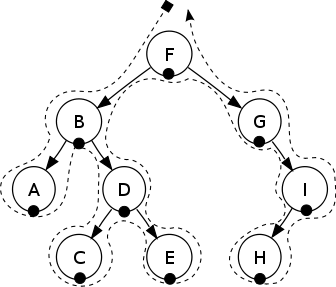
\includegraphics[width=0.50\textwidth]{sbt.png}
\end{figure}

\FloatBarrier

O percurso é feito da seguinte forma, é utilizada uma String para guardar o percurso e para cada ramo é acrescentado um zero(0) à String. Quando o nó é uma folha é acrescentado um um(1) e a seguir escreve-se na String o símbolo da folha em questão. Ignorando os nós da figura acima, excepto os nós que são folhas a String final com o percurso pós ordem é a seguinte:\\
\FloatBarrier
	"001A001C01E0001H"\\


\section{Descompressão}

Para descomprimir o ficheiro é necessário em primeiro lugar retirar o header do ficheiro mas para isso é nessário saber qual o tamanho desse header e para calcular o seu tamanho retira-se do ficheiro o tamanho do grupo utilizado, para assim calcular quantos símbolos tem a árvore. A seguir basta percorrer o ficheiro a partir do terceiro byte pois os dois primeiros são o grupo e o número de zeros acrescentados no fim do ficheiro. Ao percorrer então o ficheiro quando aparecer o bit um(1) a seguir lê-se o número de bits equivalente ao tamanho do grupo e conta-se o número de símbolos encontrados. Quando o número de símbolos encontrados for igual a 2 levantado ao tamanho do grupo significa que o Header chegou ao fim e o que vêm a seguir é o ficheiro comprimido.\\

\subsection{Reconstrução da árvore de Huffman}

\FloatBarrier
Através do percurso pós-ordem escrito no ficheiro, para reconstruir a árvore de Huffman sabe-se a à partida a ordem em que os nós são visitados, logo, quando é encontrado um um(1) o que vem a seguir é um símbolo. No que diz respeito à função para reconstruir a arvore são feitas 4 verificações, primeiro começa-se com uma lista do género - [filho esquerda, filho direita] com os dois nós filhos a null e verifica-se se o bit que estamos a observar é 0 e se o objecto que está no nó filho esquerdo é um null é chamada esta função recursivamente e avança-se um nível na arvore para o nó filho esquerdo, a mesma lógica aplica-se para o caso em que no filho direito se encontra um null. Quando se encontra um 1 coloca-se na folha um inteiro correspondente ao simbolo e o pointer avança 2 posições na bitstring. No final teremos uma lista com as sublistas que representam os diferentes niveis na arvore, em que as folhas são um inteiro que representa o simbolo.

\section{Capacidade do Canal}

Relativamente ao problema da capacidade do canal sabe-se que não há uma maneira de calcular a capacidade do canal de uma forma exacta, apenas se consegue calcular uma aproximação, por exemplo, atravéz do algoritmo de Blahut visto que a capacidade é um problema de optimização que consiste em encontrar uma distribuição p(x) tal que a informação mútua I(X;Y) seja maximizada.

\subsection{Algoritmo de Blahut}
\FloatBarrier
O algoritmo para o cálculo da capacidade de canais discretos sem memória seleccionado pelo professor foi o algoritmo de Blahut. Este algoritmo basicamente calcula a capacidade do canal iterativamente de modo a que no fim tenhamos um valor aproximado da capacidade real do canal.  Com uma distribuição de propabilidades uniforme p(x) = [$\frac{1}{n}$,$\frac{1}{n}$, ... , $\frac{1}{n}$] sendo n o número de simbolos à entrada do canal,  c{\tiny j.} os valores calculados para a capacidade ao longo das iterações do algoritmo para cada simbolo e Q{\tiny k$|$j} a matriz (transições dos estados) representativa do canal com as probabilidades de erro.\\
\FloatBarrier
A primeira coisa a ser calculada são os valores da capacidade para cada valor da distribuição de probabilidades p{\tiny j.} que neste caso é sempre igual visto tratar se de uma distribuição uniforme. De seguida vão ser calculados um limite superior e inferior indicando-nos o intervalo onde se encontra a capacidade real do canal. Se o intervalo for satisfatório, ou seja, se a diferença entre o limite superior e o limite inferior for menor que um erro $\varepsilon$ qualquer, escolhido para maximizar/minimizar a aproximação da verdadeira capacidade do canal, então definimos que o valor da capacidade é o valor calculado para o limite inferior ou para o limite superior. \\
\FloatBarrier
No programa que criamos para calcular a capacidade segundo este algoritmo adoptamos uma abordagem conservadora neste aspecto escolhendo o limite inferior para a capacidade pois se escolhessemos o limite superior para este efeito poderíamos estar a representar a capacidade com um valor maior do que o da capacidade real do canal podendo induzir em erro sendo que quanto ao limite inferior temos a certeza que a capacidade é um pouco maior que este valor. Enquanto a diferença entre os limites for maior que o erro $\epsilon$ são recalculados os valores das probabilidades de p(x) e é feita uma nova iteração do algoritmo para recalcular os limites e diminuir. O algoritmo irá continuar a recalcular os limites diminuindo o intervalo até estarmos satisfeitos com o valor obtido para a capacidade.\\
\\Colocamos varios exemplos de matrizes de cada tipo de canal que foi abordado nas aulas e há ainda hipotese de inserir qualquer outra matriz à escolha.

\section{Conclusão}

Relativamente aos dados obtidos da várias compressões que fizemos para analizar os valores conseguimos chegar a várias conclusões, como: 

{\bf }
\begin{itemize}
\item Da relação entre a entropia do ficheiro H(xt) e a entropia condicional H(xt$|$xt-1), podemos concluir que o resultado da entropia condicional é muito menor do que o resultado da entropia normal. O que nos diz que a incerteza, para quando são agrupados os bits do ficheiro orginal, é bastante mais reduzida resultando num melhor desempenho de compressão agrupando os dados, e também nos diz que os dados do ficheiro podem ser representados por uma cadeia de Markov.
\item De acordo com os resultados dos valores da taxa de compressão podemos estimar o desempenho do algoritmo de compressão para um dado grupo.
\item Podemos concluir através do calculo do comprimento médio do código L(c) o quão óptimo é o código produzido para um determinado ficheiro e grupo. Tendo em conta que o código de Huffman satisfaz a seguinte propriedade: H(X) $\leq$ $\frac{L(c)}{n}$ $<$ H(x) + $\frac{1}{n}$ em que n é o tamanho do grupo feito. O código é tanto mais óptimo quanto mais próximo estiver o comprimento médio do codigo por simbolo da entropia.  
\end{itemize}

%\includegraphics[width=0.5\textwidth]{diagrama.jpg}
%\caption{\label{fig:diagrama}This is a figure caption.}
%\end{figure}


%\begin{figure}[!htbp]
%  \caption{Como é efectuado o login do lado do servidor.}
%  \centering
%    \includegraphics[width=0.7\textwidth]{NovoServidorLogin.jpg}
%\end{figure}
\newpage


\begin{thebibliography}{9}

\bibitem{lamport94}
  Richar E. Blahut,
  \emph{Computation of Channel Capacity and Rate-Distortion functions}. IEEE TRANSACTIONS ON INFORMATION THEORY, VOL. IT-l \& NO. 4, JULHO 1972
  
\bibitem{lamport94}
  Wikipedia,
  \emph{Codificação de Huffman}. $pt.wikipedia.org/wiki/Codificacao_de_Huffman$

\end{thebibliography}


\end{document}